
\documentclass[12pt,aspectratio=169]{beamer}

% Packages
\usepackage{mathtools}
\usepackage{hyperref}
\usepackage{setspace}
\usepackage{tikz}
\usetikzlibrary{positioning}
\usepackage{ragged2e}
\usepackage{nicematrix}
\usepackage[compatibility=false]{caption}
\usepackage[framemethod=tikz]{mdframed}

% Colored boxes
\usepackage{tcolorbox}
\tcbsetforeverylayer{autoparskip} % Removes unwanted vertical space

% Theme
\usetheme{metropolis}
\metroset{subsectionpage=progressbar,sectionpage=none}
\setbeamertemplate{theorems}[numbered]

\usepackage{fontspec}
\defaultfontfeatures{LetterSpace=30}


% Code
\usepackage{listings}
% Custom colors
\definecolor{codegreen}{rgb}{0,0.6,0}
\definecolor{codegray}{rgb}{0.5,0.5,0.5}
\definecolor{codepurple}{rgb}{0.58,0,0.82}
\definecolor{backcolour}{rgb}{0.95,0.95,0.92}
\definecolor{light-gray}{gray}{0.95}
% Python style for highlighting
\newcommand\pythonstyle{\lstset{
		backgroundcolor=\color{white},
		language=Python,
		basicstyle=\ttfamily\footnotesize,
		morekeywords={self},              % Add keywords here
		keywordstyle=\color{blue},
		stringstyle=\footnotesize\color{deepgreen},
		commentstyle=\color{codegreen},
		showstringspaces=false,
		frame=tb, 
		numbers=left,
		numbersep=5pt,
		numberstyle=\tiny\color{gray},
		columns=fullflexible,
		numbersep=5pt,
		aboveskip=1em,
		showtabs=false,
		tabsize=2,
		gobble=3
}}

% Python environment
\lstnewenvironment{python}[1][]
{
	\pythonstyle
	\lstset{#1}
}
{}
% Python for inline
\newcommand\pythoninline[1]{{\pythonstyle\lstinline!#1!}}

% Tables and justification
\newcommand{\ra}[1]{\renewcommand{\arraystretch}{#1}}
\justifying

% Subfigures
\setbeamertemplate{caption}[numbered]
\usepackage[caption=false,font=footnotesize]{subfig}

% Colors
\setbeamercolor{uppercolgreen}{fg=white,bg=green!35}
\setbeamercolor{lowercolgreen}{fg=black,bg=green!10}
\setbeamercolor{uppercolred}{fg=white,bg=red!35}
\setbeamercolor{lowercolred}{fg=black,bg=red!10}
\setbeamercolor{uppercolblue}{fg=white,bg=blue!35}
\setbeamercolor{lowercolblue}{fg=black,bg=blue!10}
\definecolor{darkred}{rgb}{0.55, 0.0, 0.0}
\definecolor{darkpastelblue}{rgb}{0.47, 0.62, 0.8}
\definecolor{darkcerulean}{rgb}{0.03, 0.27, 0.49}
\definecolor{darkgreen}{rgb}{0.0, 0.55, 0.0}
\definecolor{deepblue}{rgb}{0,0,0.5}
\definecolor{deepred}{rgb}{0.6,0,0}
\definecolor{deepgreen}{rgb}{0,0.5,0}

% Matrix size
\usepackage{stackengine} 
\stackMath
\def\sss{\scriptstyle \color{gray}}
\setstackgap{L}{12pt}
\def\stacktype{L}

% Mathematical commands
\newcommand{\vc}[1]{\boldsymbol{\mathbf{#1}}}
\newcommand{\pr}[1]{{#1\,}'}
\newcommand{\idx}[2]{{\color{darkpastelblue}[}#1{\color{darkpastelblue}]_{#2}}}
\newcommand{\shape}[2]{\stackunder{#1}{\sss #2}}
\DeclareMathOperator*{\argmax}{arg\,max}
\DeclareMathOperator*{\argmin}{arg\,min}

% Style commands
\newcommand{\myalert}[1]{{\color{darkred}\textbf{#1}}}

% White frame (for images)
\newenvironment{whiteframe}[1]{
	\setbeamercolor{background canvas}{bg=white}
	\begin{frame}{#1}
	}{
	\end{frame}
}

\setbeamerfont{frametitle}{size=\normalsize}
\setbeamertemplate{frametitle}[default][right]
{	
}
%\setbeamercolor{frametitle}{fg=white,bg=black!75}

% No headline frame
\makeatletter
\newenvironment{noheadline}{
	\setbeamertemplate{headline}{}
	\addtobeamertemplate{frametitle}{\vspace*{-3.5\baselineskip}}{}
}{}
\makeatother

% Lists
\setbeamertemplate{itemize items}[triangle]

% Footnotes
\setbeamertemplate{footnote}%
{%
	\parindent 1.5em\noindent%
	\justifying\setstretch{0.7}%
	\hbox to 1em{\hfil\insertfootnotemark}\begin{scriptsize}\insertfootnotetext\end{scriptsize}\par%
}

% Footnote without number
\newcommand\blfootnote[1]{%
	\begingroup
	\renewcommand\thefootnote{}\footnote[frame]{\noindent#1}%
	\addtocounter{footnote}{-1}%
	\endgroup
}

% Theorems
\newcommand*{\theorembreak}{\usebeamertemplate{theorem end}\framebreak\usebeamertemplate{theorem begin}}
\newcounter{theo}[section]\setcounter{theo}{0}
\renewcommand{\thetheo}{\arabic{section}.\arabic{theo}}

\newenvironment{theo}[2][]{%
	\refstepcounter{theo}%
	\ifstrempty{#1}%
	{\mdfsetup{%
			frametitle={%
				\tikz[baseline=(current bounding box.east),outer sep=0pt]
				\node[anchor=east,rectangle,fill=red!10]
				{\strut Theorem~\thetheo};}}
	}%
	{\mdfsetup{%
			frametitle={%
				\tikz[baseline=(current bounding box.east),outer sep=0pt]
				\node[anchor=east,rectangle,fill=red!10]
				{\strut Theorem~\thetheo:~#1};}}%
	}%
	\mdfsetup{innertopmargin=5pt,linecolor=red!10,%
		linewidth=2pt,topline=true,%
		frametitleaboveskip=\dimexpr-\ht\strutbox\relax
	}
	\begin{mdframed}[]\relax%
		\label{#2}}{\end{mdframed}}

\usepackage{booktabs}

\begin{document}

	{\usebackgroundtemplate{\tikz\node[opacity=0.4,inner sep=0]{\includegraphics[width=\paperwidth,height=\paperheight]{images/header}};}%
	\begin{frame}[plain]
		\vspace{0.5cm}
		\title{\large \begin{spacing}{1.0}Fondamenti di Machine Learning\end{spacing}\vspace{0.25em}
			\normalsize \begin{spacing}{1.0}\textbf{Laurea Triennale in Ingegneria delle Comunicazioni}\end{spacing}\vspace{0.5em}}
		\subtitle{\Large \textbf{2: Probabilità, algebra lineare, ottimizzazione}}
		\date{
			{\includegraphics[scale=0.8]{images/Uniroma1}}
		}
		\author{
			\setlength{\tabcolsep}{2pt}
			\begin{tabular}{rl}
				\textbf{Lecturer}: & S. Scardapane \\
			\end{tabular}
		}\titlepage
	\end{frame}
	}

\part{1}

\begin{whiteframe}{Schema della lezione}
	
	\begin{figure}
		\centering\includegraphics[width=10cm,keepaspectratio]{images/Schema.pdf}
		\caption{Schema delle varie sezioni della lezione.}
	\end{figure}
	
\end{whiteframe}

\section{Algebra lineare}
\subsection{Array in NumPy}

\begin{frame}{Definizione di un array}
	
	\begin{tcolorbox}
		In NumPy, un \textbf{ndarray} (o \myalert{array}) è una collezione di oggetti dello \textit{stesso tipo} (es., interi, floating-point, caratteri). Ciascun elemento dell'array è indicizzabile con $n$ valori.
	\end{tcolorbox}
	
	Un array $X$ è descritto da:
	\begin{itemize}
		\item $n$ (a volte chiamato impropriamente \textit{rank}, o \textit{rango});
		\item il tipo dei suoi elementi (es., interi);
		\item il suo \myalert{shape}, es., $(4, 5, 2)$ è un array contenente $40$ valori.
	\end{itemize}
	
\end{frame}
	
\begin{frame}[fragile]{Inizializzare un array}
	
	Ci sono vari modi di inizializzare un array, es.:
	
	\begin{python}
		import numpy as np
		X = np.asarray([2, 1]) # Da una lista o altro oggetto Python
		X = np.random.randn(4, 5, 2) # `Random' 3-dimensional array
		X = np.zeros((3, 3)) # Matrice di soli zero
	\end{python}
	
	Nel terzo caso, la dimensione viene passata come una tupla di valori (si notino le due parentesi consecutive).
	
\end{frame}

\begin{frame}[fragile]{Indicizzazione}
	
	Estrarre singoli valori (o sottoinsiemi dell'array, \myalert{slice}) viene detto \myalert{indicizzare} l'array. Alcuni esempi:
	
	\begin{python}
		X = np.random.randn(4, 5, 2)
		X[0, 3, 1]  # Indicizzazione completa (da zero)
		X[0]		# Indicizzazione parziale (slice), di dimensioni (5, 2)
		X[0:2, 0]    # Indicizzazione parziale, di dimensioni (2, 2)
		# ...
	\end{python}
	
	Per quanto riguarda le slide, useremo $X_{i,j,k}$ o $X_{ijk}$ o $\idx{X}{i,j,k}$ per indicizzare un array, usando le stesse convenzioni che in NumPy.
	
\end{frame}

\begin{whiteframe}{Visualizzare l'indicizzazione}
	
	\begin{figure}
		\centering
		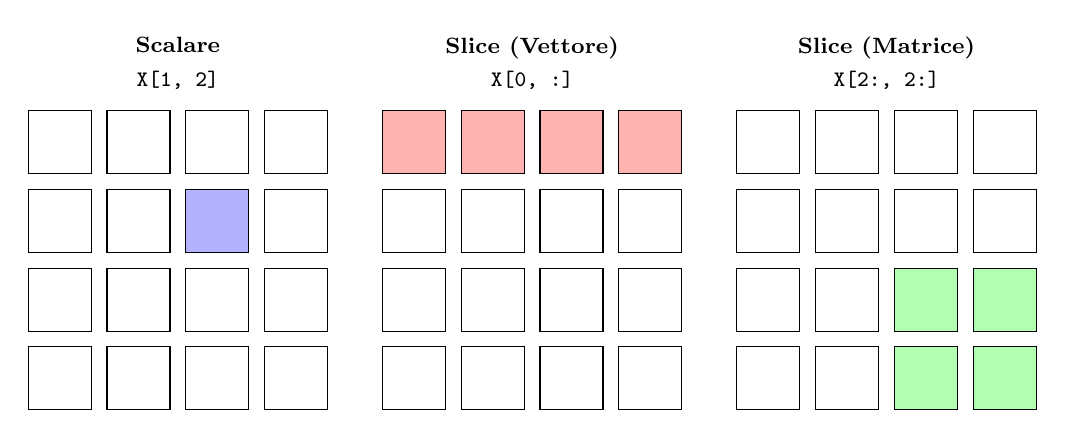
\begin{tikzpicture}
			% Define styles
			\tikzset{square/.style={draw, minimum size=0.8cm, outer sep=0pt}}
			
			% Macro to draw grid
			\def\drawgrid{
				\foreach \i in {0,...,3} \foreach \j in {0,...,3} 
				\node[square] (n-\i-\j) at (\j, -\i) {};
			}
			
			% Example 1: Scalar
			\begin{scope}[xshift=0cm]
				\drawgrid
				\node[align=center] at (1.5, 1) {\footnotesize \textbf{Scalare} \\ \footnotesize \texttt{X[1, 2]}};
				\node[square, fill=blue!30] at (2, -1) {};
			\end{scope}
			
			% Example 2: Row
			\begin{scope}[xshift=4.5cm]
				\drawgrid
				\node[align=center] at (1.5, 1) {\footnotesize \textbf{Slice (Vettore)} \\ \footnotesize \texttt{X[0, :]}};
				\foreach \j in {0,...,3} \node[square, fill=red!30] at (\j, 0) {};
			\end{scope}
			
			% Example 3: Sub-grid
			\begin{scope}[xshift=9cm]
				\drawgrid
				\node[align=center] at (1.5, 1) {\footnotesize \textbf{Slice (Matrice)} \\ \footnotesize \texttt{X[2:, 2:]}};
				\foreach \i in {2,3} \foreach \j in {2,3} 
				\node[square, fill=green!30] at (\j, -\i) {};
			\end{scope}
		\end{tikzpicture}
		\caption{Esempi visivi di operazione di indicizzazione e slicing su un array bidimensionale.}
	\end{figure}
	
\end{whiteframe}

\begin{frame}[fragile]{Broadcasting}
	
	Numerose operazioni in NumPy si applicano \textit{element-wise}, ad ogni elemento separatamente:
	%
	\begin{python}
		X = np.random.randn(4, 5)
		Y = np.random.randn(4, 5)
		Z = X + np.sin(Y) # Zij = Xij + sin(Yij)
	\end{python}
	
	A volte scriviamo operazioni che appaiono inconsistenti:
	%
	\begin{python}
		X = np.random.randn(4, 5)
		y = np.random.randn(5)
		Z = X + y # Output shape: (4, 5)
	\end{python}
	
	Questo va interpretato come $Z_i = X_i + y$ (\myalert{broadcasting}).
	
\end{frame}

\begin{frame}{Le regole del broadcasting}
	
	Il broadcasting permette di eseguire operazioni tra array di forme diverse se rispettano queste regole:
	%
	\begin{enumerate}
		\item Gli shape vengono allineati a partire da \myalert{destra} verso sinistra.
		\item Se un array ha meno dimensioni dell'altro, il suo shape viene esteso a sinistra con degli \textbf{1} (\myalert{padding}).
		\item Due dimensioni sono compatibili se:
		\begin{itemize}
			\item sono \textbf{uguali};
			\item oppure una delle due è \textbf{1}.
		\end{itemize}
	\end{enumerate}
	
	Se queste condizioni non sono verificate, NumPy solleva un \texttt{ValueError}.
	
\end{frame}

\begin{whiteframe}{Regole di broadcasting}
	
	\begin{figure}
		\centering\includegraphics[width=8cm,keepaspectratio]{images/02.05-broadcasting.png} %
		\caption{Esempi di broadcasting in NumPy.}
	\end{figure}
	
\end{whiteframe}

\begin{frame}[fragile]{Attenzione al broadcasting!}
	
	Consideriamo questa porzione di codice:
	%
	\begin{python}
		a = np.random.randn(3)
		b = np.random.randn(3)
		
		# Sum of errors squared
		e = ((a - b)**2).sum()
		
		# *WRONG* sum of errors squared
		e = ((a.reshape((3,1)) - b.reshape((1,3)))**2).sum()
	\end{python}
	%
	A causa del brodcasting, oggetti con dimensioni (3,), (3,1), o (1,3) sono fondamentalmente diversi.
	
\end{frame}

\subsection{Vettori e matrici}

\begin{frame}{Scalari e vettori}
	
	Un array $0$-dimensionale viene detto uno \myalert{scalare}. Un array $1$-dimensionale è invece, nella terminologia dell'algebra lineare, un \myalert{vettore} (e lo denotiamo in grassetto):
	%
	\begin{equation*}
		\mathbf{x} = \begin{bmatrix}
			x_1 \\ x_2 \\ \ldots \\ x_m
		\end{bmatrix} \,, \;\; \mathbf{x}^\top = \begin{bmatrix}
			x_1 & x_2 & \ldots & x_m
		\end{bmatrix}
	\end{equation*}
	%
	Possiamo interpretare un vettore come un punto nello spazio (o, equivalentemente, come il segmento che collega l'origine a quel punto).
	
\end{frame}

\begin{frame}{Operazioni sui vettori}
	
	Possiamo sommare tra loro due vettori (regola del parallelogramma):
	%
	\begin{equation*}
		\vc{z} = a\vc{x} + b\vc{y} \,, \;{z}_i = ax_i + by_i \,.
	\end{equation*}
	%
	La \textit{lunghezza} del vettore (norma $\ell_2$, la distanza dall'origine), è data da:
	%
	\begin{equation}
		\lVert \vc{x} \rVert^2 = \sum_i x_i^2 \,.
	\end{equation}
	%
	\begin{tcolorbox}
		Il  \myalert{prodotto scalare} (dot product) tra due vettori è invece dato da:
		%
		\begin{equation*}
			\langle \vc{x}, \vc{y} \rangle = \sum_i x_iy_i = \vc{x}^\top\vc{y} \,.
		\end{equation*}
	\end{tcolorbox}
	
\end{frame}

\begin{frame}{Prodotto scalare e cosine similarity}
	
	Geometricamente, il prodotto scalare è legato all'angolo $\theta$ tra i due vettori (\myalert{cosine similarity}):
	%
	\begin{equation}
		\cos(\theta) = \frac{\langle \vc{x}, \vc{y} \rangle}{\lVert \vc{x} \rVert \lVert \vc{y} \rVert} \,.
	\end{equation}
	
	Per due vettori \myalert{ortogonali}, $\langle \vc{x}, \vc{y} \rangle = 0$. Altrimenti, la cosine similarity oscilla tra $-1$ (vettori opposti) e $+1$ (vettori allineati).
	
	La norma Euclidea si può riscrivere in funzione dei prodotti scalari:
	%
	\begin{equation*}
		\lVert \vc{x} - \vc{y} \rVert_2^2 = \langle \vc{x}, \vc{x} \rangle + \langle \vc{y}, \vc{y} \rangle - 2 \langle \vc{x}, \vc{y} \rangle \,.
	\end{equation*}
	
\end{frame}

\begin{frame}{Matrici}
	Array $2$-dimensionali sono detti \myalert{matrici}:
	%
	\NiceMatrixOptions
	{code-for-first-row=\color{blue},code-for-last-col=\color{blue}}
	\begin{equation*}
		\vc{X} = 
		\begin{bNiceMatrix}[first-row,last-col=4]
			\Ldots[line-style={solid,<->},shorten=0pt]^{n \text{ columns}} & \\
			X_{1,1} & \Cdots & X_{1,n} & \\
			\Vdots & \Ddots & \Vdots & \;\;\Vdots[line-style={solid,<->},shorten=0pt]^{m \text{ rows}} \\
			X_{m,1} & \Cdots & X_{m,n} &
		\end{bNiceMatrix}
	\end{equation*}
	
	Numericamente, una matrice può essere interpretata come un \myalert{batch} (insieme) di vettori:
	%
	\begin{equation*}
		\vc{X} = \begin{bmatrix}
			\vc{X}_1 \\ \vdots \\ \vc{X}_m
		\end{bmatrix} \,, \;\;\; \vc{X} = \begin{bmatrix}
			\vc{X}_{:,1} & \dots & \vc{X}_{:,n}
		\end{bmatrix}
	\end{equation*}
	
\end{frame}

\begin{frame}{Il prodotto matrice-vettore}
	Il prodotto tra una matrice $\vc{W} \in \mathbb{R}^{m \times n}$ ed un vettore $\vc{a} \in \mathbb{R}^n$ produce un vettore $\vc{b} \in \mathbb{R}^m$:
	%
	\begin{equation*}
		\stackunder{\vc{b}}{\sss (m)} = \stackunder{\vc{W}}{\sss (m, n)} \;\; \stackunder{\vc{a}}{\sss (n)} \,.
	\end{equation*}
	%
	Ogni elemento di $\vc{b}$ è il prodotto scalare tra la riga corrispondente di $\vc{W}$ ed il vettore $\vc{a}$:
	%
	\begin{equation*}
		b_i = \langle \vc{W}_{i,:}, \vc{a} \rangle = \sum_{j=1}^n W_{ij} a_j \,.
	\end{equation*}
	%
	{\small
	\begin{tcolorbox}
		In alternativa, possiamo esprimere $\vc{b}$ come una \myalert{combinazione lineare} delle colonne di $\vc{W}$:
		%
		\begin{equation*}
			\vc{b} = \sum_{j=1}^n a_j \vc{w}_{:,j} = a_1 \vc{w}_{:,1} + \dots + a_n \vc{w}_{:,n} \,.
		\end{equation*}
	\end{tcolorbox}
	}

\end{frame}

\begin{frame}{Matrici come mappe lineari}
	Una matrice $\vc{A} \in \mathbb{R}^{m \times n}$ può essere interpretata come una \myalert{funzione} (o mappa) $f: \mathbb{R}^n \rightarrow \mathbb{R}^m$:
	%
	\begin{equation*}
		f(\vc{x}) = \vc{Ax}
	\end{equation*}
	%
	Questa mappa è \myalert{lineare}, ovvero rispetta il principio di sovrapposizione:
	%
	\begin{equation*}
		f(a\vc{u} + b\vc{v}) = a f(\vc{u}) + b f(\vc{v})
	\end{equation*}
	%
	Molte operazioni che vedremo nel corso (es. un layer di una rete neurale) sono fondamentalmente trasformazioni lineari (o quasi-lineari) di questo tipo.
\end{frame}

\begin{frame}{Column Space e Span}
	L'insieme di tutti i possibili output di una mappa lineare $f(\vc{x}) = \vc{Ax}$ viene detto l'\myalert{immagine} della funzione.
	
	Poiché $\vc{Ax}$ è una combinazione lineare delle colonne di $\vc{A}$, l'immagine coincide con lo \myalert{span} (lo spazio generato) dalle sue colonne:
	%
	\begin{equation*}
		\text{im}(\vc{A}) = \mathcal{C}(\vc{A}) = \text{span}(\vc{a}_{:,1}, \dots, \vc{a}_{:,n})
	\end{equation*}
	%
	Questo viene chiamato lo \myalert{spazio delle colonne} (column space) della matrice. Se le colonne sono linearmente indipendenti, esse formano una base per questo spazio.
\end{frame}

\begin{frame}{Moltiplicazione tra matrici}
	
	Possiamo combinare linearmente due matrici: $\vc{Z} = a\vc{X} + b\vc{Y}$. Generalizzando il prodotto scalare, possiamo anche definire una moltiplicazione tra matrici.
	
	\begin{tcolorbox}
		Il \myalert{prodotto matriciale} $\mathbf{Z}=\mathbf{X}\mathbf{Y}$ tra $\shape{\vc{X}}{(a,b)}$ e $\shape{\vc{Y}}{(b,c)}$ è definito come:
		%
		\begin{equation*}
			Z_{i,j} = \langle \vc{X}_i, \vc{Y}_{:,j} \rangle = \sum_z X_{iz}Y_{zj} \in \mathbb{R}^{a \times c}\,.
		\end{equation*}
	\end{tcolorbox}
	%
	In questa forma, ogni riga di $\vc{Z}$ è il prodotto matrice-vettore tra $\vc{X}$ ed una colonna di $\vc{Y}$, ovvero $\vc{Z}_{:,j} = \vc{X} \vc{Y}_{:,j}$.
\end{frame}

\begin{frame}[fragile]{Operazioni batched}
	
	Se consideriamo una matrice come un batch di vettori, abbiamo che:
	%
	\begin{align}
		\vc{XW} = \begin{bmatrix}
			\vc{X}_1 \\ \vdots \\ \vc{X}_m
		\end{bmatrix}\vc{W} = \begin{bmatrix}
			\vc{X}_1\vc{W} \\ \vdots \\ \vc{X}_m\vc{W}
		\end{bmatrix}
	\end{align}
	
	Una singola moltiplicazione tra matrici è equivalente ad $m$ prodotti vettori-matrici. Questo tipo di operazioni sono molto importanti in quanto le operazioni in NumPy sono estremamente ottimizzate rispetto ad, es., un for-loop.
	
	Un altro esempio: $\vc{X}\vc{X}^\top$ è una matrice contenente tutti i prodotti scalari $\langle \vc{X}_i, \vc{X}_j \rangle$.
	
\end{frame}

\section{Teoria delle probabilità}

\subsection{Regole base della probabilità}

\begin{frame}{Un primo esempio}
	
	Consideriamo questo esempio (riprodotto da Bishop, 2006):
	
	\begin{figure}
		\centering\includegraphics[width=4cm,keepaspectratio]{images/Figure1.9.pdf}
		\caption{Abbiamo due scatole con diverse proporzioni di palline \textbf{arancioni} e \textbf{verdi}, provenienti da due scatole (\textbf{rossa} e \textbf{blu}). Possiamo chiederci ``\textit{Qual è la probabilità di estrarre una pallina verde?}'', oppure ``\textit{Qual è la probabilità di aver estratto dalla prima scatola, dato che il colore della pallina è arancione?}''.}
	\end{figure}
	
\end{frame}

\begin{frame}{Probabilità come frequenze}
	
	Definiamo una variabile $C$ che può prendere i valori \textit{verde} ed \textit{arancione}. La probabilità che una pallina estratta sia di un dato colore è data da:
	%
	\begin{align}
	p(C = \text{`verde'}) = 5 / 12 \\
	p(C = \text{`arancione'}) = 7/12
	\end{align}
	%
	$p(C)$ definisce una \textit{distribuzione di probabilità} sui valori di $C$, e rispetta le seguenti proprietà:
	%
	$$
	p(C = c) \ge 0, \,\, \sum_{c} p(C = c) = 1 \,.
	$$
	%
	Questa viene detta l'intepretazione \textit{frequentista} della probabilità.
	
\end{frame}

\begin{frame}{Distribuzione di probabilità congiunta}
	
	Ora consideriamo una seconda variabile, $B$, che descrive la scatola (\textit{blu} o \textit{rossa}). Una \myalert{distribuzione di probabilità congiunta} coinvolge le due variabili insieme:
	%
	$$
	p(C = \text{`verde'}, B = \text{`blu'}) = 2 / 12.
	$$
	%
	La \textit{regola della somma} delle probabilità ci permette di \textit{marginalizzare} (rimuovere) una delle due variabili:
	%
	$$
	p(C=c) = \sum_{b} p(C=c, B = b) \,.
	$$
	%
	Ad esempio, $p(C = \text{`verde'}) = p(C = \text{`verde'}, B = \text{`rossa'}) + p(C = \text{`verde'}, B = \text{`blu'}) = 2/12 + 3/12 = 5/12$.
	
\end{frame}

\begin{frame}{Probabilità condizionali}
	
	La \myalert{distribuzione di probabilità condizionale} $p(C \mid B)$ definisce la probabilità di osservare una variabile aleatoria $C$ se conosciamo il valore di un'altra variabile $B$. Ad esempio (sempre contando le palline):
	%
	$$
	p(C = \text{`verde'} \mid B = \text{`rossa'}) = 2 / 8.
	$$
	%
	La \textit{regola del prodotto} delle probabilità mette in relazioni le probabilità congiunte e condizionali:
	%
	$$
	p(C=c, B=b) = p(B=b)P(C=c\mid B=b) = p(C=c)p(B=b \mid C=c) \,.
	$$

\end{frame}

\begin{frame}{Una notazione abbreviata}
	
	Possiamo semplificare la notazione evitando di scrivere esplicitamente i valori delle variabili. Ricapitolando tutti gli assiomi fondamentali di una distribuzione di probabilità:
	%
	\begin{align*}
		p(C) \ge 0 & & \texttt{\small [Una probabilità è sempre positiva]} \\
		\sum_C p(C) = 1 & & \texttt{\small [La somma delle probabilità è 1]} \\
		p(C) = \sum_{B} p(C, B) & & \texttt{\small [Regola della somma]} \\
		p(C, B) = p(B)P(C\mid B) & & \texttt{\small [Regola del prodotto]}
	\end{align*}

\end{frame}

\begin{frame}{Regola di Bayes}
	%
	Se $p(C,B) = p(C)p(B)$, $C$ e $B$ sono dette \textbf{indipendenti}. 
	
	Combinando invece la regola della somma e del prodotto, otteniamo la \myalert{regola di Bayes}:
	%
	$$
	p(B \mid C) = \frac{p(C \mid B)p(B)}{p(C)} \,.
	$$
	%
	Dove $p(C)=\sum_B p(C \mid B)p(B)$. Possiamo interpretare questa regola in vari modi: tra le altre cose, ci permette di aggiornare la nostra conoscenza di $B$ data da $p(B)$ dopo aver osservato un evento $C$.
	
\end{frame}

\subsection{Distribuzioni di probabilità continue}

\begin{frame}{Definizione nel caso continuo}
	
	Consideriamo ora il caso di una variabile $x$ che può assumere valori continui (es., l'altezza di una persona). In questo caso, possiamo definire una \myalert{funzione di densità di probabilità} (\myalert{probability density function}) $p(x)$ definita come:
	%
	\begin{equation}
		p(x \in [a,b]) = \int_a^b p(x)dx \,.
	\end{equation}
	%
	Tale funzione deve rispettare:
	%
	$$
	p(x) \ge 0, \,\, \int p(x)dx = 1 \,.
	$$
	
\end{frame}

\begin{frame}{Distribuzione di probabilità cumulativa}
	
	In particolare, la \myalert{distribuzione di probabilità cumulativa} (\myalert{cumulative probability distribution}) è data da:
	%
	\begin{equation}
		P(x) = \int_{-\infty}^x p(y)d(y) 
	\end{equation}
	%
	da cui $p(x) = P'(x)$. Riotteniamo le regole viste prima in maniera simile:
	%
	\begin{align}
	p(x) = \int p(x \mid y)p(y)dy \\
	p(x, y) = p(x \mid y)p(y) \\
	p(y \mid x) = \frac{p(x \mid y)p(y)}{\int_y p(x \mid y)p(y)dy }
	\end{align}
	
\end{frame}
	
\begin{frame}{Funzioni di densità e cumulative}
	
	\begin{figure}
		\centering\includegraphics[width=7cm,keepaspectratio]{images/Figure1.12.pdf}
		\caption{Riprodotta da (Bishop e Bishop, 2023).}
	\end{figure}
	
\end{frame}

\subsection{Manipolare le probabilià}

\begin{frame}{Valori attesi}
	
	Il \myalert{valore atteso} di una funzione $f(x)$ è dato da:
	%
	$$
	\mathbb{E}[f(x)] = \sum_{x} f(x)p(x) \,.
	$$
	%
	In particolare, la \myalert{media} è il valore atteso di $f(x)=x$:
	%
	\begin{equation*}
		\mathbb{E}[x] = \sum_{x} xp(x)
	\end{equation*}
	%
	Ad esempio, se vinciamo $x=1$ per palline verdi e $x=2$ per palline arancioni, la vincita media è data da $\mathbb{E}[x]=5/12 + 2*7/12\approx 1.6$.
	
\end{frame}

\begin{frame}{Varianza}

	La \myalert{varianza} di $x$ è invece definita come lo spostamento quadratico medio rispetto alla media:
	%
	\begin{equation}
		\text{Var}(x) = \mathbb{E}\left[(x - \mathbb{E}\left[x\right])^2\right] = \mathbb{E}[x^2] - \mathbb{E}[x]^2
	\end{equation}
	%
	Ritornando all'esempio delle palline, la varianza ci permette di calcolare quanto potrebbero variare le nostre vincite individuali su varie ripetizioni.

\end{frame}

\begin{frame}{Proprietà del valore atteso}

	Il valore atteso ha due proprietà fondamentali:
	%
	\begin{itemize}

		\item \myalert{Linearità}: $\mathbb{E}[aX + b] = a\mathbb{E}[X] + b$ \,, per ogni $a, b \in \mathbb{R}$ .
		\item \myalert{Additività}: $\mathbb{E}[X + Y] = \mathbb{E}[X] + \mathbb{E}[Y]$ \,, anche se $X$ e $Y$ \myalert{non sono indipendenti}.

	\end{itemize}

	Queste proprietà rendono il valore atteso molto semplice da manipolare nei modelli di ML, dove spesso lavoriamo con somme di variabili casuali.

\end{frame}

\begin{frame}{Esempio: lancio di due dadi}

	Se lanciamo due dadi equi $D_1$ e $D_2$, qual è la somma attesa $S = D_1 + D_2$?
	%
	\begin{itemize}
		\item Sappiamo che $\mathbb{E}[D_1] = \mathbb{E}[D_2] = \frac{1+2+3+4+5+6}{6} = 3.5$.
		\item Per l'additività:
		      \begin{equation*}
			      \mathbb{E}[D_1 + D_2] = \mathbb{E}[D_1] + \mathbb{E}[D_2] = 3.5 + 3.5 = 7 \,.
		      \end{equation*}
	\end{itemize}

	Nota bene: non abbiamo avuto bisogno di calcolare la tabella di probabilità di tutte le 36 possibili combinazioni della somma!

\end{frame}

\begin{frame}{Covarianza e Correlazione}

	La \myalert{covarianza} misura quanto due variabili $x$ e $y$ variano insieme:
	%
	\begin{equation}
		\text{Cov}(x, y) = \mathbb{E}\left[(x - \mathbb{E}[x])(y - \mathbb{E}[y])\right] = \mathbb{E}[xy] - \mathbb{E}[x]\mathbb{E}[y]
	\end{equation}
	%
	Se $x$ e $y$ sono indipendenti, $\text{Cov}(x, y) = 0$.

	Spesso normalizziamo la covarianza per ottenere la \myalert{correlazione} $\rho \in [-1, 1]$:
	%
	\begin{equation*}
		\rho_{xy} = \frac{\text{Cov}(x, y)}{\sqrt{\text{Var}(X)\text{Var}(Y)}}
	\end{equation*}

\end{frame}

\begin{frame}{Esempio: dipendenza tra variabili}

	\begin{center}
		\small
		\begin{tabular}{cccc}
			\toprule
			Città & Temp. ($X$) & Gelati ($Y$) & Termosifoni ($Z$) \\
			\midrule
			A     & 10          & 100          & 500               \\
			B     & 20          & 200          & 300               \\
			C     & 30          & 300          & 100               \\
			\bottomrule
		\end{tabular}
	\end{center}

	\begin{itemize}
		\item $X$ e $Y$ hanno \textbf{covarianza positiva} (al crescere della temperatura crescono i consumi di gelato).
		\item $X$ e $Z$ hanno \textbf{covarianza negativa} (al crescere della temperatura diminuiscono i riscaldamenti).
	\end{itemize}

\end{frame}

\begin{frame}{Proprietà della varianza}

	A differenza del valore atteso, la varianza \myalert{non è lineare}:
	%
	\begin{itemize}
		\item $\text{Var}(aX + b) = a^2\text{Var}(X)$ \,.
		\item $\text{Var}(X + Y) = \text{Var}(X) + \text{Var}(Y) + 2\text{Cov}(X, Y)$ \,.
	\end{itemize}

	Se $X$ e $Y$ sono indipendenti (e quindi $\text{Cov}(X,Y)=0$), la varianza della somma è la somma delle varianze.

	\begin{tcolorbox}
		\textbf{Esempio numerico}: Se triplichiamo una variabile ($Y=3X$), la sua varianza aumenta di \textbf{9 volte}.
	\end{tcolorbox}

\end{frame}

\begin{frame}{Stimare la media di una distribuzione}
	
	Supponiamo di non avere accesso a $p(x)$ (non possiamo guardare dentro le scatole), ma possiamo campionare valori $x \sim p(x)$ (estrarre una pallina). Con un sufficiente numero di campioni possiamo stimare il valore atteso:
	%
	\begin{equation}
		\mathbb{E}[f(x)] = \sum_{x} f(x)p(x) \approx \frac{1}{n}\sum_{i=1}^n f(x_i)
	\end{equation}
	%
	dove $x_1, \ldots, x_n$ sono i campioni. Questo viene detto \myalert{metodo di Monte Carlo}.
	
\end{frame}

\subsection{Distribuzioni di probabilità parametriche}

\begin{frame}{One-of-$k$ encoding}
	
	Un concetto che useremo ripetutamente è quello di \myalert{one-hot encoding} (o \myalert{one-of-$k$ encoding}, o \myalert{dummy encoding}). 
	
	Consideriamo una variabile discreta $x \in \left\{1, \ldots, k\right\}$. Il suo one-hot encoding è un vettore $\mathbf{x} \in \left\{0,1\right\}^k$ tale che:
	%
	\begin{equation}
		x_i = \begin{cases} 1 & \text{ se } x=i \\
		0 & \text{ altrimenti} \end{cases}
	\end{equation}
	
\end{frame}

\begin{frame}{Esempio di dummy encoding}
	
	Consideriamo $x \in \left\{`verde', `blu', `arancione'\right\}$. L'encoding diventa:
	%
	\begin{equation}
		`verde' = \begin{bmatrix} 1 \\ 0 \\ 0 \end{bmatrix} ,\;\; `blu' = \begin{bmatrix} 0 \\ 1 \\ 0 \end{bmatrix} ,\;\; `arancione' = \begin{bmatrix} 0 \\ 0 \\ 1 \end{bmatrix}
	\end{equation}
	%
	Il dummy encoding permette di trasformare una variabile categorica in un vettore, senza imporre un ordinamento tra gli elementi.
	
\end{frame}

\begin{frame}{Distribuzioni categoriche}
	
	Raggruppiamo le probabilità associate ad $x$ in un vettore $\mathbf{p} = \left[p_1, \ldots, p_k\right]^\top$. Possiamo descrivere l'intera distribuzione di probabilità in maniera concisa come:
	%
	\begin{equation}
		\text{Cat}(\mathbf{x} ; \mathbf{p}) = \prod_{i=1}^k p_i^{x_i} = p_1^{x_1}p_2^{x_2} \cdots p_k^{x_k} \,,
	\end{equation}
	%
	dove $\mathbf{x}$ è il dummy encoding di $x$. Scritta in questa forma, viene detta una \myalert{distribuzione categorica}. La notazione $\text{Cat}(x ; \mathbf{p})$ chiarisce che $\mathbf{p}$ sono gli unici parametri necessari a specificare interamente la distribuzione stessa: vengono detti \myalert{sufficient statistic}.
	
\end{frame}

\begin{frame}{Distribuzione Gaussiana}
	
	Nel caso di variabili aleatorie continue, una distribuzione molto comune è quella \myalert{Gaussiana}:
	%
	\begin{equation}
		p(x) = \mathcal{N}(x;\mu,\sigma^2)= \frac{1}{\sqrt{2\pi \sigma^2}}\exp\left(-\frac{1}{2}\left(\frac{x-\mu}{\sigma}\right)^2\right)
	\end{equation}
	%
	Questa rappresenta una distribuzione centrata in $\mu$ (la \myalert{media}), che decresce sui lati in maniera simmetrica con uno spread che dipende da $\sigma^2$ (la \myalert{varianza} della distribuzione).
	
\end{frame}

\begin{frame}{Visualizzazione della distribuzione Gaussiana}
	
	\begin{figure}
		\centering\includegraphics[width=7cm,keepaspectratio]{images/Figure1.13.pdf}
		\caption{Riprodotto da (Bishop e Bishop, 2023).}
	\end{figure}
	
\end{frame}

\subsection{Maximum likelihood}

\begin{frame}{Maximum likelihood}
	
	Supponiamo di non conoscere $p(x)$, ma di avere accesso ad $n$ campioni $\left\{{x}_i\right\}, {x}_i \sim p({x})$.
	
	Abbiamo però l'intuizione che la distribuzione abbia una forma $f({x}; {s})$, di cui non conosciamo però le statistiche sufficienti ${s}$. Il principio del \myalert{maximum likelihood} (massima verosimiglianza) ci permette di stimare questi valori, se assumiamo che essi siano stati campionati in maniera indipendente l'uno dall'altro.
	
\end{frame}

\begin{frame}{Maximum likelihood}
	
	Essendo i campioni indipendenti, possiamo scrivere una distribuzione congiunta fattorizzata:
	%
	\begin{equation}
		p(x_1, \ldots, x_n)=\prod_{i=1}^n f(x_i; s) 
	\end{equation}
	%
	Banalmente, i parametri ottimi sono quelli che massimizzano questa quantità:
	%
	\begin{equation}
		s^*=\underset{s}{\arg\max} \prod_{i=1}^n f(x_i;s)
	\end{equation}
	
\end{frame}

\begin{frame}{Log likelihood}
	
	Se $n$ è grande, produttorie di tantissimi elementi possono essere instabili a livello numerico. In questo caso, possiamo definire la \myalert{log-likelihood} come il logaritmo della likelihood:
	%
	\begin{equation}
		\log p(x_1, \ldots, x_n) = \sum_{i=1}^n \log f(x_i; s)
	\end{equation}
	%
	Poiché il logaritmo è monotono, massimizzare la log-likelihood è equivalente a massimizzare la likelihood:
	%
	\begin{equation}
		s^*= \underset{s}{\arg\max} \sum_{i=1}^n \log f(x_i;s)
	\end{equation}
	
\end{frame}

\begin{frame}{ML per una distribuzione categorica}
	
	Vedremo più avanti che possiamo risolvere problemi di ottimizzazione di questo tipo tramite \myalert{discesa al gradiente}. Consideriamo prima due esempi semplici di stima ML (per le derivazioni si veda (Bishop e Bishop, 2023)).\footnote{Come spoiler dalla prossima sezione: possiamo massimizzare la likelihood imponendo che all'ottimo il suo gradiente sia uguale a zero.}
	
	Consideriamo una distribuzione categorica. Otteniamo:
	%
	\begin{equation}
		p_i = \frac{\sum_{j=1}^n \idx{x_i}{j}}{n}
	\end{equation}
	%
	che non è altro che la frazione di valori $i$ osservati tra gli $n$ campionati.

\end{frame}

\begin{frame}{ML per una Gaussiana}
	
	Consideriamo ora una Gaussiana. Possiamo riscrivere la log-likelihood come:
	%
	\begin{equation}
		L(\mu, \sigma^2) = - \frac{n}{2}\log(2\pi \sigma^2) - \frac{1}{2\sigma^2}\sum_{i=1}^n(x_i-\mu)^2
	\end{equation}
	%
	Da cui otteniamo (utile esercizio provarci):
	%
	\begin{align}
		\mu^*=\frac{1}{n}\sum_i x_i \\ \sigma^{2*}=\frac{1}{n}\sum_i(x_i-\mu^*)^2
	\end{align}
	
\end{frame}

\begin{frame}{Maximum likelihood per una Gaussiana}
	
	\begin{figure}
		\centering\includegraphics[width=7cm,keepaspectratio]{images/Figure1.14.pdf}
		\caption{Riprodotta da (Bishop e Bishop, 2023). Trovare la media ottima (secondo il principio della massima verosimiglianza) vuol dire scegliere $\mu$ tale da minimizzare il quadrato della somma dei segmenti verdi.}
	\end{figure}
	
\end{frame}

\section{Ottimizzazione numerica}
\subsection{Derivate e gradienti}

\begin{frame}{Derivata di una funzione}
	
	Consideriamo una funzione $f(x): \mathbb{R} \rightarrow \mathbb{R}$. Sotto certe condizioni, possiamo studiarne l'andamento tramite la sua derivata.
	
	\begin{tcolorbox}
		La \myalert{derivata} di una funzione $f(x)$ è definita come:
		%
		\begin{equation}
			\partial f(x) = \pr{f}(x) = \lim_{h \rightarrow 0} \frac{f(x+h) - f(x)}{h} \,.
		\end{equation}
		%
		Anche per una funzione continua, non è detto che la derivata sia definita ovunque.
	\end{tcolorbox}

	La derivata descrive come varia $f(x)$ per uno spostamento `infinitesimo' rispetto ad $x$.
	
\end{frame}

\begin{frame}{Esempi di derivate}
	
 	Derivata di un polinomio:
	%
	\[
		\partial \left[ x^p \right] = px^{p-1} \,.
	\]
	
	Derivata di funzioni esponenziali e logaritmi:
	%
	\begin{gather*}
		\partial \left[ \exp(x) \right] = \exp(x) \,, \\
		\partial \left[ \log(x) \right] = \frac{1}{x} \,.
	\end{gather*}
	
\end{frame}


\begin{frame}{Proprietà delle derivate}
	
	Le derivate possiedono numerose proprietà algebriche, tra cui:
	%
	\begin{itemize}
		\item \textbf{Linearità}: $$ \partial \Big[{\color{darkred}f(x)} + {\color{darkgreen}g(x)}\Big] = {\color{darkred}\pr{f}(x)} + {\color{darkgreen}g'(x)} \,. $$
		\item \textbf{Regola del prodotto}: $$ \partial\Big[ {\color{darkred}f(x)}{\color{darkgreen}g(x)}\Big] = {\color{darkred}\pr{f}(x)}{\color{darkgreen}g(x)} + {\color{darkred}f(x)}{\color{darkgreen}g'(x)} \,, $$
		\item \textbf{Chain rule (regola della composizione)} $$ \partial \Big[{\color{darkred}f(}{\color{darkgreen}g(x)}{\color{darkred})}\Big] = {\color{darkred}\pr{f}(}{\color{darkgreen}g(x)}{\color{darkred})}{\color{darkgreen}g'(x)} \,. $$
	\end{itemize}		
	
\end{frame}

\begin{whiteframe}{Visualizzare la derivata}
		
	\begin{figure}
	\centering\includegraphics[width=8cm,keepaspectratio]{../scripts/gradient_info.pdf} %
	\caption{$f(x) = x^2 - 1.5x$. La derivata in ogni punto può essere interpretata come la pendenza della linea tangente in quel punto.}
	\end{figure}
		
\end{whiteframe}


\begin{frame}{Gradienti}
	
	Per una funzione $y=f(\vc{x})$, $\vc{x} \in \mathbb{R}^m$, il \myalert{gradiente} $\partial f(\vc{x})$ è un vettore $m$-dimensionale:%
	\begin{equation}
		\idx{\partial f(\vc{x})}{i} = \frac{\partial y}{\partial x_i} = \lim_{h \rightarrow 0} \frac{f(\vc{x} + h\vc{e}_i) - f(\vc{x})}{h} \,,
	\end{equation}
	%
	dove $\vc{e}_i$ è il vettore:
	%
	\begin{equation*}
		\idx{\vc{e}_i}{j} = \begin{cases} 1 & \text{ se } i=j \\ 0 & \text{altrimenti} \end{cases}
	\end{equation*} 
	%
	A volte useremo la notazione $\nabla f(\vc{x})$ per indicare il gradiente.
	
\end{frame}

\begin{frame}{Derivata direzionale}
	
	\begin{tcolorbox}
	Più in generale, la \myalert{derivata direzionale} di $f(\vc{x})$  lungo una direzione $\vc{v}$ è data da:
	%
	\begin{equation}
		\mathrm{D}_{\vc{v}}f(\vc{x}) = \lim_{h \rightarrow 0} \frac{f(\vc{x} + h\vc{v}) - f(\vc{x})}{h} \,,
	\end{equation}
	\end{tcolorbox}
	%
	Si può provare la seguente identità (informalmente, il movimento si decompone rispetto agli assi):
	%
	\begin{equation}
		\mathrm{D}_{\vc{v}}f(\vc{x}) = \langle \nabla f(\vc{x}), \vc{v} \rangle \,.
	\end{equation}

\end{frame}

\begin{frame}{Gradienti e Jacobiani}
	
	Nel caso più generale $\vc{y} = f(\vc{x})$, $\vc{x} \in \mathbb{R}^m$, $\vc{y} \in \mathbb{R}^n$:
	%
	\begin{tcolorbox}
		Lo \myalert{Jacobian} $\stackunder{\partial f(\vc{x})}{\sss (n, m)}$ di $f$ è definito come:
		%
		\begin{equation}
			\partial f(\vc{x}) = \begin{pmatrix}
				\frac{\partial y_1}{\partial x_1} & \dots & \frac{\partial y_1}{\partial x_m} \\
				\vdots & \ddots & \vdots \\
				\frac{\partial y_n}{\partial x_1} & \dots & \frac{\partial y_n}{\partial x_m} \\
			\end{pmatrix} \,.
		\end{equation}
	\end{tcolorbox}
	%
	Per $n=1$ otteniamo il gradiente, per $m = n = 1$ otteniamo la derivata.
	
\end{frame}

\begin{frame}{Esempi di Jacobiani e gradienti}
	
    Prodotto scalare:
	%
	\[
	\frac{\partial}{\partial \vc{x}} \langle \vc{x}, \vc{y} \rangle = \vc{y} \,.
	\]
	
	Moltiplicazione di un vettore e di una matrice:
	%
	\[
	\frac{\partial}{\partial \vc{x}} \vc{A}\vc{x} = \vc{A} \,.
	\]
	
	Gradiente della norma:
	%
	\[
	\partial \lVert \vc{x} \rVert^2 = 2\vc{x} \,.
	\]
	
	\blfootnote{Si veda come riferimento: \\ \url{https://www.math.uwaterloo.ca/~hwolkowi/matrixcookbook.pdf}.}
	
\end{frame}

\begin{frame}{Proprietà dei gradienti}
	
	Quasi tutte le regole delle derivate si estendono al caso multi-variato, ad esempio (linearità):
	%
	\begin{equation}
		\partial(f(\mathbf{x}) + g(\mathbf{x})) = \partial f(\mathbf{x}) + \partial g(\mathbf{x})
	\end{equation} 
	
	Esiste anche una chain rule: date $f: \mathbb{R}^m \rightarrow \mathbb{R}^n$ e $g: \mathbb{R}^o \rightarrow \mathbb{R}^m$, con $\mathbf{h}= g(\mathbf{x})$:
	%
	\begin{equation}
		\stackunder{\partial \left[ f(g(\mathbf{x})) \right]}{\sss (n,o)} = \stackunder{\partial f(\mathbf{h})}{\sss (n,m)} \stackunder{\partial g(\mathbf{x})}{\sss (m,o)} \,.
	\end{equation}
	%
	In parole: lo Jacobiano della composizione è il prodotto (matriciale) dei due Jacobiani individuali.
	
\end{frame}

\begin{frame}{Approssimazione al primo ordine}
	
	Data una funzione $f(\vc{x}_0)$ valutata in $\vc{x}_0$, la funzione:
	%
	\begin{equation}
		\widetilde{f}(\vc{x}) = f(\vc{x}_0) + \langle \partial f(\vc{x}_0), \vc{x} - \vc{x}_0 \rangle
	\end{equation}
	%
	è la miglior \textbf{approssimazione lineare} di $f$ rispetto a $\vc{x}_0$ (\myalert{teorema di Taylor}). Considerando derivate di ordini superiori è possibile migliorare la qualità dell'approssimazione.
	
\end{frame}

\begin{frame}[fragile]{Un esempio con il codice}
	
	\begin{python}
	 # Function
	 f = lambda x: x**2 - 1.5*x
	
	 # Derivative (manual)
	 df = lambda x: 2*x - 1.5
	
	 # Linearization at 0.5
	 x = 0.5
	 f_linearized = lambda h: f(x) + df(x)*(h - x)
	
	 print(f(x + 0.01))             # -0.5049
	 print(f_linearized(x + 0.01))  # -0.5050
	\end{python}
	
\end{frame}

\begin{whiteframe}{Visualizzazione}
	
	\begin{figure}
		\centering\includegraphics[width=8cm,keepaspectratio]{../scripts/taylor_approximation.pdf} %
		\caption{Funzione ($f(x) = x^2 - 1.5x$), linearizzata in 0.5.}
	\end{figure}
	
\end{whiteframe}

\subsection{Discesa al gradiente}

\begin{frame}{Ottimizzare una funzione}
	
	Consideriamo nuovamente un problema di questo tipo:
	%
	\begin{equation}
		\vc{x}^* = \argmin_{\vc{x} \in \mathbb{R}^d} f(\vc{x})
	\end{equation}
	%
	Si tratta di un problema di \myalert{ottimizzazione (non vincolata)} nel dominio $\mathbb{R}^d$. Massimizzare rispetto a minimizzare è una scelta stilistica, in quanto:
	%
	\begin{equation}
		\vc{x}^* = \argmax_{\vc{x} \in \mathbb{R}^d} f(\vc{x}) = \argmin_{\vc{x} \in \mathbb{R}^d} {\color{darkred} -} f(\vc{x})
	\end{equation}
	%
	Il maximum likelihood è un esempio di tale problema (se la likelihood è differenziabile).

\end{frame}

\begin{frame}{Minimi e massimi di una funzione}
	
	\begin{tcolorbox}
		Un punto $\vc{x}$ per il quale $f(\vc{x}) \le f(\vc{x}') \;\;\forall\; \vc{x}' \in \mathbb{R}^d$ viene detto un \myalert{minimo globale}. In maniera meno restrittiva, invece, se:
		%
		\begin{equation}
			f(\vc{x}) \le f(\vc{x}') \;\;\forall\; \vc{x}' \in \left\{ \vc{x}': \lVert \vc{x}' - \vc{x} \rVert^2 < \varepsilon \right\}
		\end{equation}
		%
		per qualche $\varepsilon > 0$, allora il punto viene detto un \myalert{minimo locale}.
	\end{tcolorbox}
	
	\begin{tcolorbox}
		Se $\nabla f(\vc{x}) = 0$, $\vc{x}$ il punto viene detto \myalert{stazionario}. Come vedremo, i punti stazionari possono essere minimi, massimi, oppure \myalert{punti di sella}.
	\end{tcolorbox}
	
\end{frame}

\begin{whiteframe}{Classi di punti stazionari}
		
	\begin{figure}
	\centering\includegraphics[width=8cm,keepaspectratio]{images/Extrema_example_original.png} %
	\vspace{-1em}\caption{Senza nessuna informazione aggiuntiva, un punto stazionario può essere un \myalert{minimo}, un \myalert{massimo}, e può essere \myalert{locale} o \myalert{globale} (\textit{Wikimedia, KSmrq}).}
	\end{figure}
		
\end{whiteframe}

\begin{whiteframe}{Punti di sella}
		
	\begin{figure}
	\centering\includegraphics[width=8cm,keepaspectratio]{../scripts/saddle_point.pdf} %
	\vspace{-0.5em}\caption{I punti stazionari possono essere anche \myalert{punti di sella}, che crescono e decrescono in direzioni diverse.}
	\end{figure}
		
\end{whiteframe}

\begin{frame}{Trovare punti stazionari}
	
	Consideriamo un punto (scelto casualmente) $\vc{x}_0$, ed un algoritmo iterativo in cui ad ogni istante ci muoviamo in una direzione $\vc{p}_t$ per una lunghezza $\eta_t$:
	%
	\begin{equation}
		\vc{x}_t = \vc{x}_{t-1} + \eta_t \vc{p}_t \,.
	\end{equation}
	%
	\begin{tcolorbox}
		$\vc{p}_t$ è chiamata una \myalert{descent direction} in $f(\vc{x}_{t-1})$ se $f(\vc{x}_t) < f(\vc{x}_{t-1})$ per qualche $\eta_t$, anche molto piccolo. $\eta_t$ viene detto \myalert{step size} o \myalert{learning rate}.
	\end{tcolorbox}
	
\end{frame}

\begin{frame}{Descent direction}
	
	Poiché $\vc{p}_t$ descrive solo la direzione del movimento, possiamo assumere che $\lVert \vc{p}_t \rVert = 1$. Possiamo quantificare il cambiamento (infinitesimo) dello spostamento con la derivata direzionale:
	%
	\begin{equation*}
		\mathrm{D}_{\vc{p}_t} f(\vc{x}_{t-1}) = \langle \nabla f(\vc{x}_{t-1}), \vc{p}_t \rangle = \lVert \nabla f(\vc{x}_{t-1}) \rVert \underbrace{\lVert \vc{p}_t \rVert}_{=1} \cos(\theta) = \lVert \nabla f(\vc{x}_{t-1}) \rVert \cos(\theta).
	\end{equation*}
	%
	Dall'equazione si vede che la discesa è massima quando $\cos(\theta) = -1$, cioè quando $\theta=\pi$ e $\vc{p}_t = - \nabla f(\vc{x}_{t-1})$. Questa viene chiamata la \myalert{steepest descent direction}. In generale, qualsiasi direzione tale per cui $\cos(\theta) < 0$ è una descent direction.
	
\end{frame}

\begin{frame}{Discesa al gradiente}
	
	Un algoritmo iterativo in cui scegliamo sempre di muoverci nella steepest descent direction viene detto \myalert{discesa al gradiente}.
	%
	\begin{tcolorbox}
		La discesa al gradiente trova un punto stazionario di una funzione $f(\cdot)$ tramite la seguente procedura iterativa:
		%
		\begin{equation}
		\vc{x}_t = \vc{x}_{t-1} - \eta_t \nabla f(\vc{x}_{t-1}) \,.
	\end{equation}
	\end{tcolorbox}
	
\end{frame}

\begin{frame}{Definizione di una funzione convessa}
	
	Il concetto di \myalert{convessità} è essenziale nell'ottimizzazione. Se una funzione è convessa, la sua ottimizzazione è più semplice in quanto non esistono minimi locali. 
	
	\begin{tcolorbox}
	$f$ è convessa se per $\lambda \in [0,1]$:
	
	\begin{equation}
	f\Bigl((1-\lambda)\vc{x}_1 + \lambda \vc{x}_2\Bigr) \le (1-\lambda)f(\vc{x}_1) + \lambda f(\vc{x}_2) \,.
	\end{equation}
	\end{tcolorbox}
		
	Se questo vale sempre in maniera stretta, $f$ viene detta \myalert{strettamente convessa} (strictly convex).
	
\end{frame}

\begin{frame}{Visualizzazione della convessità di una funzione}
	
	\begin{figure}
		\centering\includegraphics[width=7cm,keepaspectratio]{./images/Figure1.31.pdf}
		\caption{Riprodotto da (Bishop e Bishop, 2023).}
	\end{figure}
	
\end{frame}

\begin{whiteframe}{Funzioni convesse e non convesse}
		
	\begin{figure}
	\centering\includegraphics[width=11cm, keepaspectratio]{images/Convex_non_convex_functions.png}
	\caption{Sinistra: un esempio di funzione convessa. Destra: un esempio di funzione non convessa. Riprodotto da ``An Introduction to Machine Learning'' by Smola and Vishwanathan [unpublished].}
	\end{figure}
		
\end{whiteframe}

\begin{frame}{Convessità ed ottimizzazione}
	
	\begin{tcolorbox}
	Consideriamo una funzione $f(\vc{x})$, e supponiamo la discesa al gradiente converga ad un punto $\vc{x}^*$. Allora:
	%
	\begin{itemize}
		\item \textbf{Se $f(\vc{x})$ è non convessa}: il punto è \textbf{stazionario}.
		\item \textbf{Se $f(\vc{x})$ è convessa}: il punto è un \textbf{minimo globale}.
		\item \textbf{Se $f(\vc{x})$ è strettamente convessa}: il punto è \textbf{l'unico} minimo globale.
	\end{itemize}
	\end{tcolorbox}
	%
	Per una funzione non convessa questo risultato non può essere migliorato (informalmente: l'unico modo di trovare un ottimo globale è inizializzare la discesa al gradiente da \textit{qualsiasi} punto dello spazio).
	
\end{frame}

\end{document}
